\documentclass[utf8,hyperref={unicode,pdftex}]{beamer}
%\documentclass[utf8]{beamer}

\mode<presentation>
{
\usetheme{Warsaw}
}
\setbeamertemplate{navigation symbols}{}

\usepackage[utf8]{inputenc}
\usepackage[L7x]{fontenc}
\usepackage[lithuanian]{babel}
\usepackage{lmodern}
\usepackage{amsmath}
\usepackage{amssymb}
\usepackage{bm}
\usepackage{graphicx}
\usepackage{multirow}

\beamersetuncovermixins{\opaqueness<1>{25}}{\opaqueness<2->{15}}

\title[\hspace{130pt} p. \insertpagenumber\enspace iš \insertdocumentendpage\enspace ]{HLM modeliai TIMSS duomenims:\\ Duomenys}
\author[ E. Kaleckaitė]{Eglė Kaleckaitė}
\institute{Vilniaus Universitetas, Matematikos ir Informatikos Fakultetas}
\date{2013 spalio 16d.}
\begin{document}
\begin{frame}
\titlepage
\end{frame}
\begin{frame}
\frametitle{Turinys}
\Large
\begin{enumerate}
\item Įvadas
\item TIMSS klausimynų ir imčių sudarymas
\item Užduočių pavyzdys
\item Duomenų apdorojimas
\item Stuktūra
\item Darbo tikslas
\item Kas šioje srityje jau nuveikta
\end{enumerate}
\end{frame}
%\section{Įvadas}
\begin{frame}
\frametitle{Įvadas}
\begin{itemize}
\item TIMSS - Tarptautinis matematikos ir gamtos mokslų tyrimas (\textit{angl. Trends in International Mathematics and Science Study})
\item Pagrindiniai klausimai: kas, ko ir kaip yra mokoma klasėse, ką mokiniai išties išmoksta ir kaip jie įgytas žinias vertina?
\item IEA - Tarptautins švietimo pasiekimų vertinimo asociacija (\textit{angl. International Association of the Evaluation of Educational Achievement})
\item Apie 70 šalių
\item Dar vykdoma PIRLS, ICCS , SITES, TEDS-M ir ICILS.
\end{itemize}
\end{frame}
%\section{Duomenys}
%\subsection*{Duomenys}
\begin{frame}
\frametitle{TIMSS klausimynų ir imčių sudarymas}
\begin{itemize}
\item Šalių skirtumai
\item Tyrimo medžiaga:
\begin{itemize}
\item Testo sąsiuviniai
\item Klausimynas apie mokymo programas
\item Mokinio klausimynas
\item Mokytojo klausimynas
\item Mokyklos klausimynas
\end{itemize}
\item TIMSS imtis yra dviejų pakopų sluoksninė lizdinė, kurios pirmos pakopos elementai išrenkami su tikimybėmis, proporcingomis dydžiui, antos pakopos elementai išrenkami su lygiomis tikimybėmis.
\end{itemize}
\end{frame}

\begin{frame}
\frametitle{Pavyzdys}
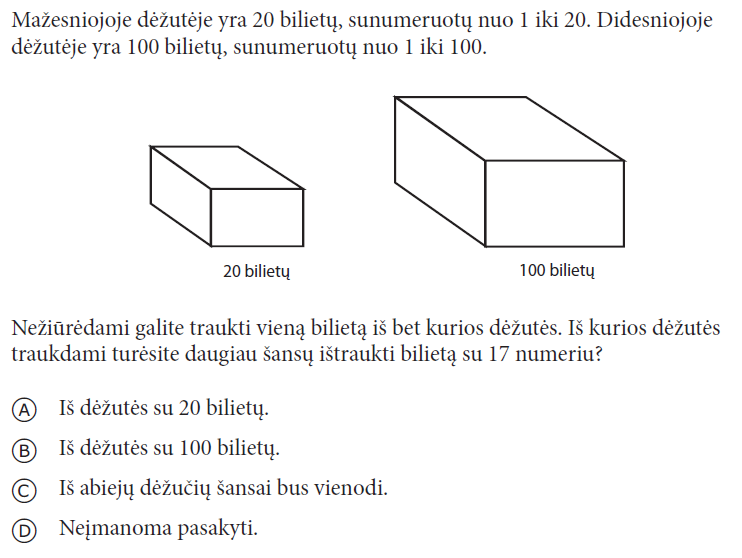
\includegraphics[height=8.5cm]{uzdPvz1.png}
\end{frame}

\begin{frame}
\frametitle{Duomenų apdorojimas - atsižvelgimas į imtis}
Mokinių svoriai:
\begin{Large}
\begin{equation}
W_i = \frac{1}{p_i}\times \frac{n}{n_i} \times \frac{C_i}{c_i} \times \frac{k_i}{k_{pi}},
\end{equation}
\end{Large}
čia $p_i$ - mokyklos išrinkimo tykimybė, $n$ - išrinktų mokyklų skaičius, $n_p$ - tyrime dalyvavusių mokyklų skaičius, $C_i$ - aštuntų klasių skaičius mokykloje, $c_i$ - išrinktų dalyvauti tyrime klasių skaičius, $k_i$ - išrinktos klasės mokinių skaičius, $k_{pi}$ - tyrime dalyvavusių mokinių skaičius.
\end{frame}

\begin{frame}
\frametitle{Duomenų apdorojimas - atsižvelgimas į ribotą laiką}
\begin{large}
\textbf{Matematinio raštingumo rezultatų galimos reikšmės (\textit{angl. Plausible values}).}
\end{large}
Atsižvelgiant į mokinio atsakytus klausimus sudaromas atskiras skirstinys kiekvienam mokiniui ir sugeneruojamos 5 galimos reikšmės.
\end{frame}

\begin{frame}
\frametitle{Struktūra}
Duomeys pateikiami kiekvieniems metams atskirai 7 (.sav ar .dat) failuose:
\begin{itemize}
\item Mokyklos
\item Mokinio rezultatų
\item Mokinio aplinkos
\item Užduočių
\item Mokytojo/Klasės aplinkos
\end{itemize}
\end{frame}

\begin{frame}
\frametitle{Magistro darbo tikslas}
\Large
Sudaryti modelį Lietuvos mokinių matematikos raštingumo pasiekimus veikiantiems veiksniams nustatyti ir įvertinti. Gautus rezultatus palyginti su kitomis šalimis.
\end{frame}

\begin{frame}
\frametitle{Kas jau nuveikta šioje srityje}
\begin{Large}
\begin{itemize}
\item Dudaitė J. (2009). \textit{Mokinių matematinio raštingumo kaita edukacinės ir mokymosi aplinkų aspektu}. Daktaro disertacija. Socialiniai mokslai, Edukologija, 07 S. Kaunas: Kauno technologijos universitetas. 
\item Akyuz G., Berberoglu G. (2010). \textit{Teacher and Classroom Characteristics and Their Relations to Mathematics Achievement of the Students in the TIMSS}. Middle East Technical University
\end{itemize}
\end{Large}
\end{frame}

\begin{frame}
\frametitle{Dudaitės sudaryti modeliai}
HLM modeliai buvo sudaryti atskirai kiekvienam kintamajam:
\[ \left\{
  \begin{array}{l l}
    Y_{ij} = \beta_{0j}+r_{ij}; \\
    \beta_{0j} = \gamma_{00} + \gamma_{01}\times X_{j}+u_{0j};
  \end{array} \right.\]
\small
čia $i$ - žymi $i$-tajį mokinį,\\
$j$ - $j$-tają mokyklą/klasę/mokytoją,\\
$Y_{ij}$ - $i$-tojo mokinio iš $j$-tosios mokyklos/klasės/mokytojo matematinio raštingumo rezultatas,\\
$\beta_{0j}$ - $j$-tosios mokyklos/klasės/mokytojo įnašas,\\
$r_{ij}$ - pirmo lygio paklaidos,\\
$\gamma_{00}$ - vidutinis mokyklų/klasių/ mokytojų įnašas,\\
$\gamma_{01}$ - vidutinis mokyklų/klasių/ mokytojų nuolydis,\\
$X_j$ - antro lygio kintamasis, \\
$u_{0j}$ - antro lygio paklaidos.
\end{frame}

\begin{frame}
\frametitle{Akyuz ir Berberoglu sudarytas modelis}
Šie autoriai sudarė tik vieną modelį:
\[ \left\{
  \begin{array}{l}
    Y_{ij} = \beta_{0j}+\beta_{1j}\times X_{ij}+r_{ij}; \\
    \beta_{0j} = \gamma_{00} + \gamma_{01}\times W_{1j}+\dots+\gamma_{0m}\times W_{mj}+u_{0j};\\
    \beta_{1j} = \gamma_{10} + u_{1j};
  \end{array} \right.\]
\small
čia $i$ - žymi $i$-tajį mokinį,\\
$j$ - $j$-tają mokyklą/klasę/mokytoją,\\
$Y_{ij}$ - $i$-tojo mokinio iš $j$-tosios mokyklos/klasės/mokytojo matematinio raštingumo rezultatas,\\
$\beta_{0j}$ - $j$-tosios mokyklos/klasės/mokytojo įnašas,\\
$\beta_{1j}$ - atsitiktinis nuolydis,\\
$X_{ij}$ - pirmo lygio kintamasis, šiuo atveju, namų edukaciniai ištekliai, \\
$r_{ij}$ - pirmo lygio paklaidos,\\
$\gamma_{00}$ - vidutinis mokyklų/klasių/ mokytojų įnašas,\\
$\gamma_{01}$ - vidutinis mokyklų/klasių/ mokytojų nuolydis,\\
$W_{mj}$ - antro lygio kintamasis, \\
$u_{0j}$ - atsitiktinis efektas,\\
$u_{1j}$ - atsitiktinis efektas.
\end{frame}

\begin{frame}
\frametitle{Pabaiga}
\LARGE
Ačiū už dėmesį :)
\end{frame}

\end{document}

